\chapter{Descrizione dell'architettura ROS}
\label{cha:descrizionearchros}
Nei capitoli precedenti abbiamo approfondito Prolog e l'applicazione del caso di studio. In questo capitolo verrà descritta l'architettura ROS utilizzata per la simulazione e la possibile applicazione reale.
In particolare verrà data una breve descrizione di cosa è ROS e come funziona, per poi passare alla descrizione dell'architettura utilizzata per la simulazione. Iniziamo quindi con una breve introduzione a ROS.

\section{Introduzione a ROS}
\label{sec:introduzione_ros}
ROS (Robot Operating Systems) è un framework opensource per lo sviluppo e la programmazione di robot. ROS implementa drivers e algoritmi che sono lo stato dell'arte in robotica grazie anche alla community che negli anni si è formata e ingrandita.
Essendo infatti un progetto opensource, ROS è sviluppato e mantenuto dalla community stessa. Questo è un grosso vantaggio infatti così facendo il supporto verso nuovi hardware sarà sempre al passo con i tempi, oltre a questo la community è molto attiva per consigli e aiuti sia per i meno esperti che non.
Per realizzare questo capitolo mi sono documentato dalla wiki del progetto \cite{rossite} e dall'articolo \textit{ROS: an open-source Robot Operating System} \cite{inproceedings}.

Iniziamo questa sezione introducendo i concetti principali di un architettura ROS: i nodi, i topic e i messaggi.

\subsection{Nodi}
\label{subsec:nodi}
Con il termine nodo si intende un processo che esegue un compito specifico, questo utilizza ROS per comunicare con gli altri nodi. Solitamente questo utilizza un ROS client library, ne identifichiamo 2: \textit{roscpp} che è l'implementazione in c++ e \textit{rospy} che è la medesima implementazione in python. I nodi possono pubblicare oppure iscriversi ad un topic, inoltre possono offrire un servizio o richiederlo. 

In ROS1, quello che è stato utilizzato per la simulazione, è necessario che ci sia un nodo master. Per avviarlo è necessario digitare il comando \verb+roscore+. Questo avrà il compito di coordinare le attività del nostro sistema distribuito. Più in dettaglio dovrà: tenere traccia dei nomi dei nodi ecc. tramite il registro dei nomi, fornire un servizio di ricerca consultabile dai nodi stessi, tenere traccia dei topic e dei messaggi che vengono pubblicati e infine fornire il servizio del parameter server.
I messaggi e le chiamate di servizio non passano dal nodo master, infatti la comunicazione in ROS è peer-to-peer. Questo permette di avere un sistema distribuito e scalabile. Inoltre, essendo peer-to-peer, non è necessario che tutti i nodi siano attivi contemporaneamente, infatti è possibile che un nodo si sottoscriva ad un topic anche se il nodo che lo pubblica non è ancora attivo. Questo permette di avere un sistema molto flessibile e scalabile.

\subsection{Topics}
\label{subsec:topics}
In ROS i topic sono un canale di comunicazione asincrona che permetta ai nodi di scambiarsi messaggi. I Topic in ROS seguono l'architettura \textit{publisher-subscriber}, un nodo quindi può pubblicare messaggi su un topic specifico mentre uno o più nodi si sottoscrivono al topic per ricevere i messaggi.
I topic in ROS sono organizzati gerarchicamente e sono identificati da un nome univoco. La gerarchia permette di organizzare i topic in base diversi aspetti dell'applicazione o dei dati che vengono scambiati. 
Come detto prima la comunicazione è asincrona, quindi il nodo pubblicante non aspetta una risposta immediata dal nodo abbonato.
Con il comando \verb+rostopic list+ possiamo avere una panoramica dei topic che sono attivi nella nostra rete. Con il comando \verb+rostopic echo <nometopic>+, invece, possiamo vedere i messaggi che vengono pubblicati su un topic specifico. In questo modo possiamo capire se i topic sono attivi e quindi se i nodi stanno comunicando tra di loro.
\subsection{Messaggi}
\label{subsec:messaggi}
I messaggi sono i dati che vengono scambiati dai nodi attraverso i topic. Questi possono essere di vari tipi e sono definiti in un file \verb+.msg+. Questo file contiene la definizione del messaggio, ovvero il nome del messaggio e i campi che lo compongono. I campi possono essere di vari tipi, come ad esempio: interi, stringhe, array, ecc.
La personalizzazione dei messaggi permette all'utente un controllo totale della propria applicazione riuscendo a definire i messaggi che meglio si adattano alle proprie esigenze.
Con il comando \verb+rostopic info <nometopic>+ possiamo avere una panoramica dei messaggi che vengono scambiati su un topic specifico. Inoltre con il comando \verb+rosmsg show <nomemsg>+ possiamo avere i dettagli di come è composto il messaggio specifico.
\subsection{ROS services e parameter server}
\label{subsec:servandparam}
L'ultima nozione fondamentale da sapere sull'architettura ROS è il concetto di \textit{ROS service} e \textit{parameter server}. I ROS service sono un modo alternativo per comunicare in ROS, questi a differenza dei topic sono sincroni. Questo significa che il nodo che richiede un servizio deve aspettare che il nodo che lo fornisce risponda. 
Anche i ROS services sono identificati da un nome univoco e vengono chiamati/richiesti appunto da esso. Una volta che un nodo richiede un servizio questo bloccherà la sua esecuzione, riprendendola solamente quando il servizio sarà stato fornito.
I servizi in ROS vengono usati principalmente se è necessario ottenere una risposta immediata, ad esempio la richiesta di dati di configurazione, l'esecuzione di operazioni complesse oppure la richiesta di operazioni specifiche.

Il \textit{parameter server} in ROS è un componente centrale che consente ai nodi di memorizzare e recuperare dei parametri di sistema. Può essere inteso come un database centralizzato in cui i nodi possono leggere e scrivere i valori dei parametri.
Questi parametri possono essere usati per configurare il comportamento dei nodi, impostare valori costanti o condividere dati tra i componenti del sistema. I parametri sono organizzati tramite dei namespace così da semplificare la ricerca e la gerarchia.

\subsection{Esempio rete ROS}
\label{subsec:esempio_rete_ros}
Per capire meglio come sono strutturati questi componenti utilizziamo il famoso simulatore \textit{turtlesim} e generiamo il grafo della rete tramite il comando \verb+rosrun rqt_graph rqt_graph+. Il grafo generato è il seguente
\begin{figure}[h!]
    \centering
    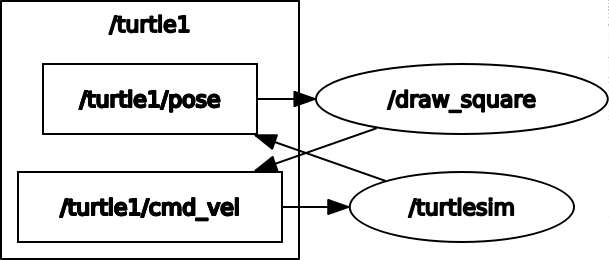
\includegraphics[scale=0.5]{images/turtlesim.png}
    \caption{Grafo della rete turtlesim}
    \label{fig:turtlesim}
\end{figure}
I nodi sono identificati dagli ovali mentre i topic sono identificati dai rettangoli. Vediamo come i due nodi: turtlesim e draw\_square comunicano tra loro tramite i topic \verb+/turtle1/pose+ e \verb+/turtle1/cmd_vel+. Il nodo /draw\_square pubblica sul topic /cmd\_vel la traiettoria per la "tartaruga", questa sarà poi inviata al nodo del simulatore per poi essere eseguita. Quest'ultimo a sua volta pubblicherà la posa del robot al topic /pose che sarà poi letto dal nodo /draw\_square per recuperare la posizione del robot e disegnare la traiettoria.
\begin{figure}[h!]
    \centering
    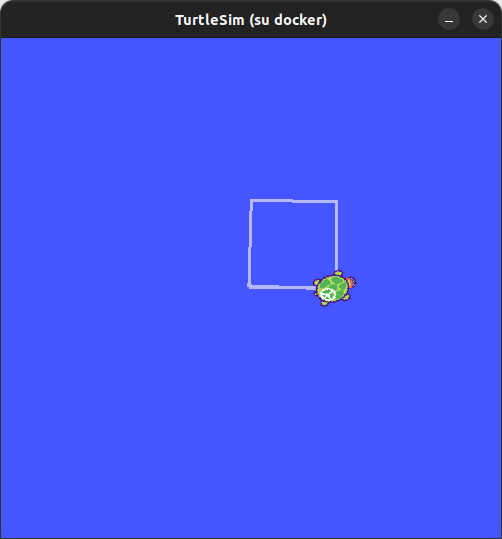
\includegraphics[scale=0.4]{images/turtlesimes.png}
    \caption{Esempio di simulazione turtlesim}
    \label{fig:turtlesimes}
\end{figure}
\section{Architettura utilizzata}
\label{sec:architettura_utilizzata}

